\documentclass{article}
\usepackage[utf8]{inputenc}
\usepackage{geometry}
\usepackage{datetime2}
\usepackage{xparse}
\usepackage{amsmath}
\usepackage{booktabs}
\usepackage{array}
\usepackage{hyperref}
\usepackage{indentfirst}
\usepackage{float}
\usepackage{tabularx}

 \geometry{
 a4paper,
 total={170mm,257mm},
 left=20mm,
 top=20mm,
 }

 
 \usepackage{graphicx}
 \usepackage{titling}

 \title{Assignment: Simulasi Rangkaian IZCD \& NIZCD with Hysteresis
}
% \author{Faizal Fitrohni}
\date{18 March 2025}
 
 \usepackage{fancyhdr}
\fancypagestyle{plain}{%  the preset of fancyhdr 
    \fancyhf{} % clear all header and footer fields
    \fancyfoot[R]{}
    \fancyfoot[L]{}
    \fancyhead[L]{
\includegraphics[width=2cm]{ITS_pojok.pdf}}
    \fancyhead[R]{ \DTMnow}
}
\makeatletter
\def\@maketitle{%
  \newpage
  \null
  \vskip 1em%
  \begin{center}%
  \let \footnote \thanks
    {\LARGE \@title \par}%
    \vskip 1em%
    %{\large \@date}%
  \end{center}%
  \par
  \vskip 1em}
\makeatother

\usepackage{lipsum}  
% \usepackage{cmbright} % Change the font by zee

\begin{document}

\maketitle

\noindent\begin{tabular}{@{}ll}
    Author(s): & Faizal Fitrohni\\
     Teacher: &  Muhammad Qomaruz Zaman, S.T., M.T., Ph.D.\\
     Class name: & Rangkaian Analog\\
     YouTube video link: & \url{https://youtu.be/mE_aMZ2CNZk?si=dWNSuZegymR0buQy} \\
     GitHub link: & \url{}
\end{tabular}
\vspace{2cm}

\section*{Positive Feedback}

Umpan balik positif (\textit{positive feedback}) terjadi saat sebagian sinyal output dikembalikan ke terminal non-inverting (+) op-amp, yang secara sengaja memperkuat perbedaan tegangan input untuk memaksa output segera berpindah (switching) ke kondisi saturasi. Meskipun rangkaian komparator biasanya berkaitan dengan op-amp open loop, tetapi karena fungsi utamanya tetap untuk membandingkan level tegangan input terhadap suatu ambang batas guna menghasilkan output logika biner (Tinggi/Rendah), maka positive feedback juga disebut sebagai rangkaian comparator, khususnya comparator dengan hysteresis.

Hysteresis memberikan dua ambang batas tegangan yang berbeda:

\begin{itemize}
    \item \textbf{Upper Threshold} ($V_{UT}$): Tegangan yang harus dilewati agar output berubah dari rendah ke tinggi.
    \item \textbf{Lower Threshold} ($V_{LT}$): Tegangan yang harus dilewati agar output berubah dari tinggi ke rendah.
\end{itemize}

Begitu sinyal input melewati $V_{UT}$, ambang batas akan "bergeser" secara otomatis menjadi $V_{LT}$. Dengan adanya jarak antara $V_{UT}$ dan $V_{LT}$ (yang disebut Hysteresis Band), gangguan kecil pada sinyal tidak akan cukup kuat untuk memicu perubahan output yang tidak diinginkan.

\subsection*{Inverting Zero Crossing Detector with Hysteresis }

\subsubsection*{Penjelasan IZCD with Hysteresis}

Rangkaian IZCD menggunakan Op-amp yang dikonfigurasikan sebagai pembanding (comparator). Pada konfigurasi ini, Op-amp tidak bekerja di area linier, melainkan selalu berada pada kondisi saturasi \cite{pujiono2012rangkaian}. Oleh karena itu, tegangan keluaran ($V_o$) hanya memiliki dua kemungkinan nilai:

\begin{itemize}
    \item $+V_{sat}$ (Tegangan saturasi positif)
    \item $-V_{sat}$ (Tegangan saturasi negatif)
\end{itemize}

Ketika rangkaian diaktifkan, output akan berada pada salah satu kondisi saturasi. Hal ini menyebabkan munculnya tegangan referensi pada kaki (+) akibat pembagi tegangan resistor $R_1$ dan $R_2$.

\begin{enumerate}
    \item [a. ]\textbf{Upper Threshold Voltage ($V_{UT}$)}
    
    Terjadi saat $V_o = +V_{sat}$. Tegangan ini adalah batas atas yang harus dilalui sinyal input agar output berubah.
    $$V_{UT} = \left( \frac{R_2}{R_1 + R_2} \right) (+V_{sat})$$
    
    \item [b. ]\textbf{Lower Threshold Voltage ($V_{LT}$)}
    
    Terjadi setelah output berpindah ke $-V_{sat}$. Ini adalah batas bawah yang harus dilalui sinyal input agar output kembali ke positif.
    $$V_{LT} = \left( \frac{R_2}{R_1 + R_2} \right) (-V_{sat})$$
\end{enumerate}

\subsubsection*{Simulasi IZCD with Hysteresis}
\begin{enumerate}
    \item [a. ]$R_1 = R_2$
        \begin{figure}[H]
        \centering
        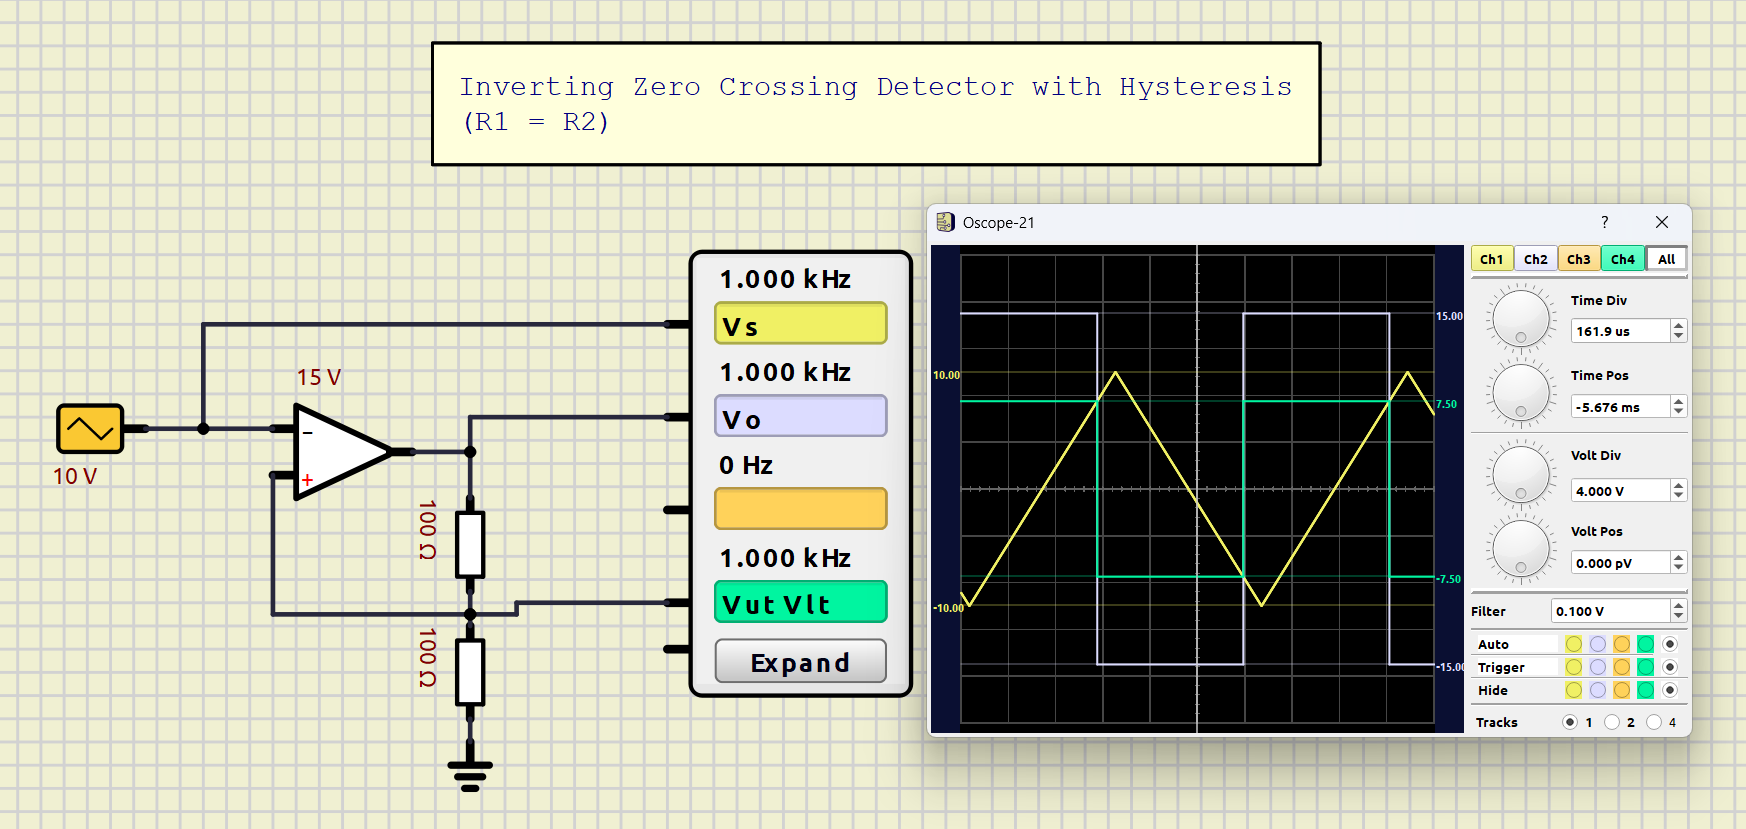
\includegraphics[width=0.5\linewidth]{images/IZCD1.png}
        \caption{IZCD with Hysteresis $R_1 = R_2$}
        \end{figure}
    
    \item [b. ]$R_1 < R_2$
        \begin{figure}[H]
        \centering
        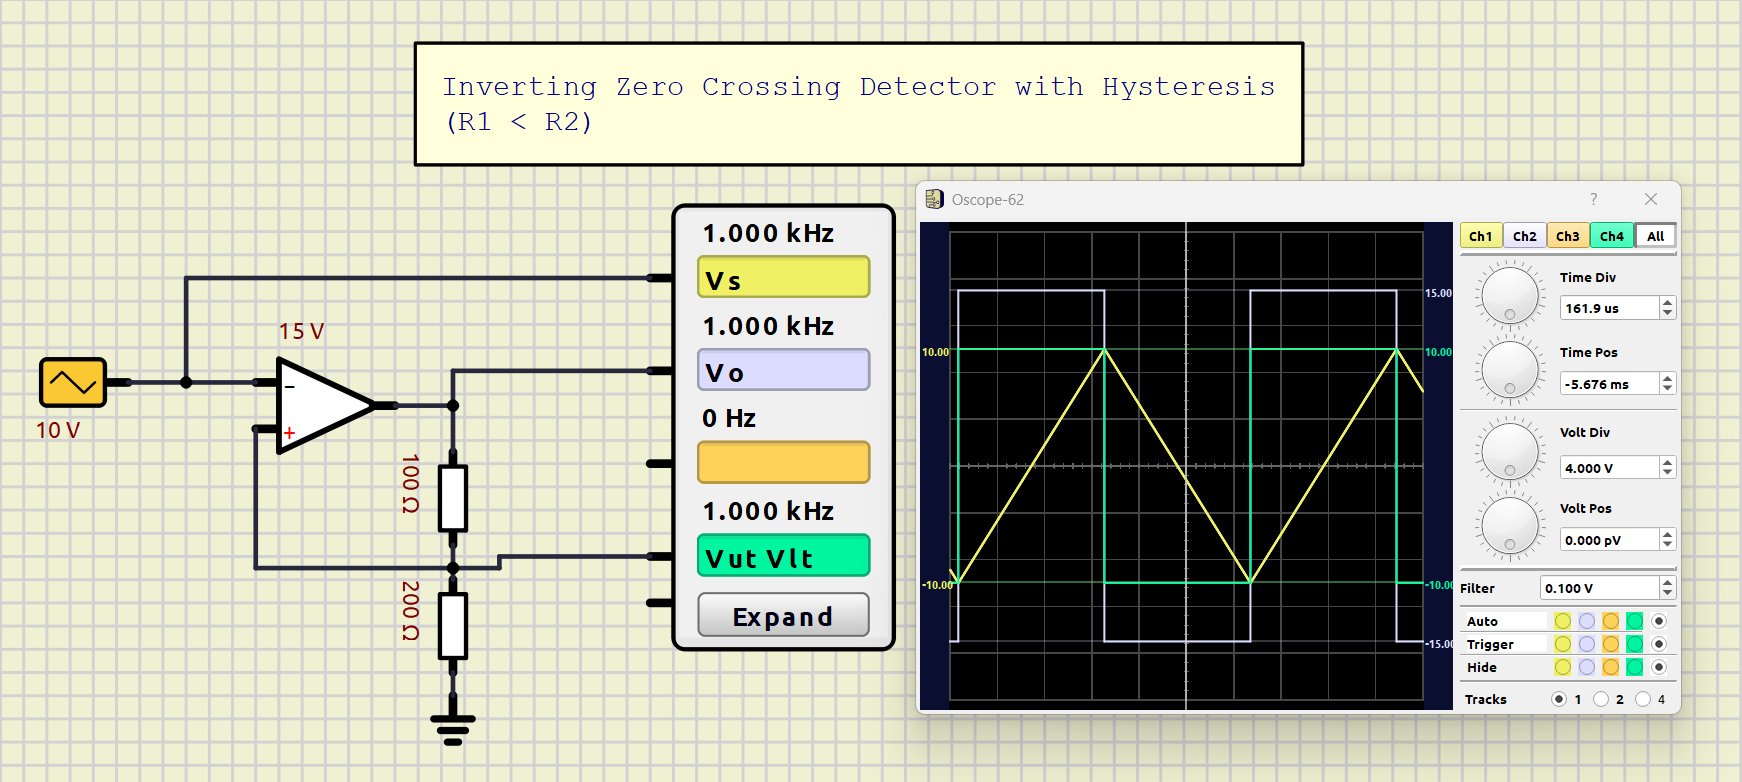
\includegraphics[width=0.5\linewidth]{images/IZCD2.png}
        \caption{IZCD with Hysteresis $R_1 < R_2$}
        \end{figure}
    
    \item [c. ]$R_1 > R_2$
        \begin{figure}[H]
        \centering
        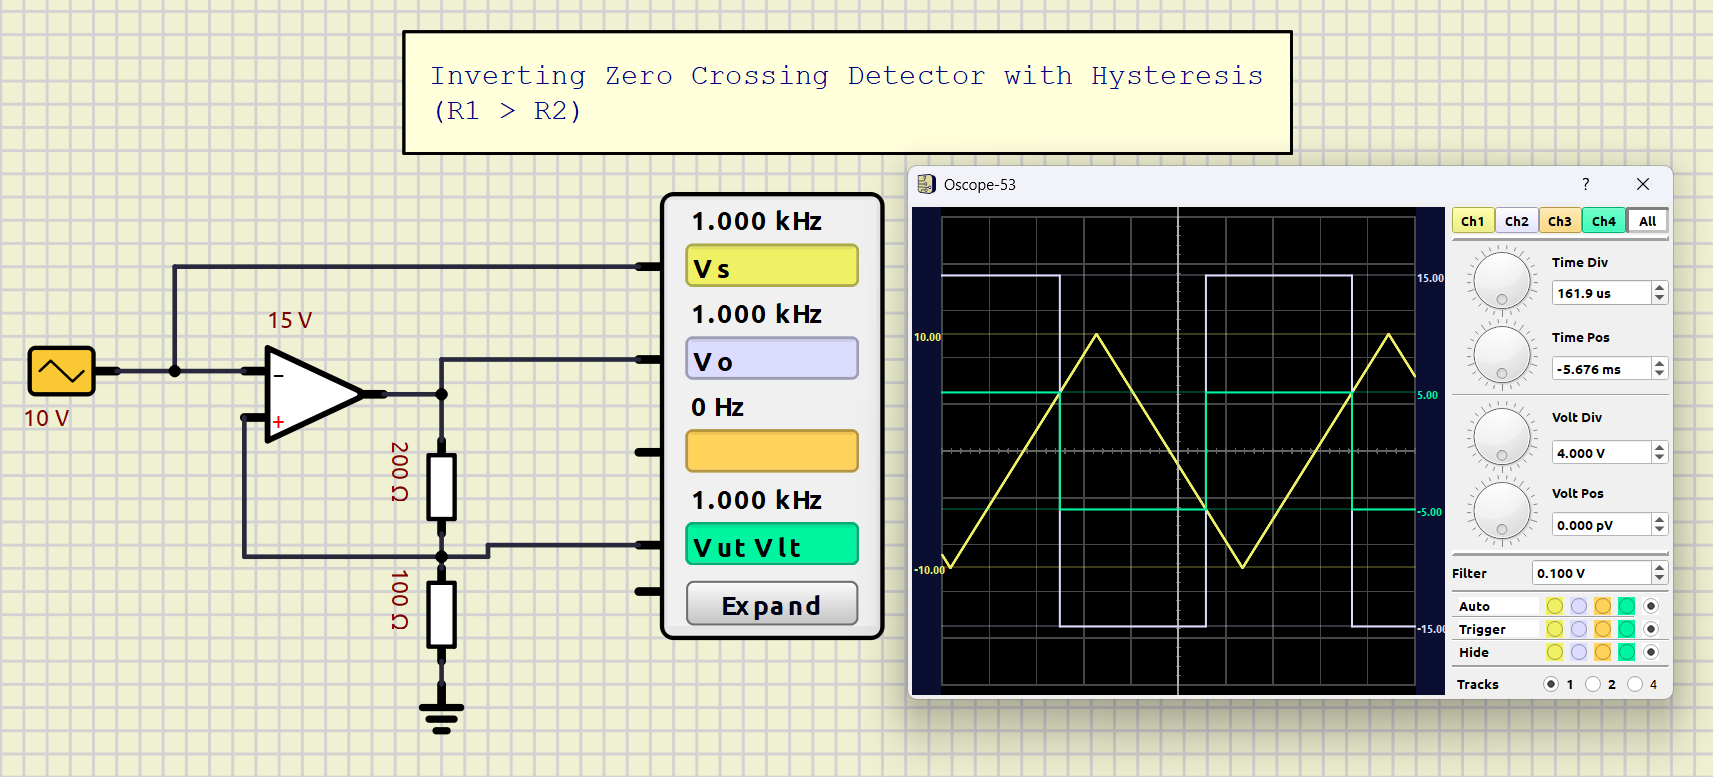
\includegraphics[width=0.5\linewidth]{images/IZCD3.png}
        \caption{IZCD with Hysteresis $R_1 > R_2$}
        \end{figure}
    
\end{enumerate}

Pada simulasi ini, perbandingan nilai resistor $R_1$ dan $R_2$ secara langsung menentukan lebar jendela histerisis dan karakteristik pemicuan output. Ketika $R_1 > R_2$ ($200\Omega / 100\Omega$), dihasilkan threshold yang sempit sebesar $\pm 5V$ sehingga output ($V_o$) berpindah lebih cepat karena posisi ambang batas yang dekat dengan titik nol, namun kondisi ini membuatnya lebih sensitif terhadap gangguan noise. Sebaliknya, pada kondisi $R_1 = R_2$ ($100\Omega / 100\Omega$), jendela histerisis melebar menjadi $\pm 7.5V$ yang memberikan perlindungan lebih baik terhadap noise dengan titik transisi yang tepat berada di setengah tegangan saturasi. Terakhir, pada skenario $R_1 < R_2$ ($100\Omega / 200\Omega$), rangkaian memiliki threshold paling lebar mencapai $\pm 10V$ yang menjadikannya paling kebal terhadap gangguan, meskipun mengakibatkan keterlambatan perpindahan output karena sinyal input membutuhkan waktu lebih lama untuk mencapai ambang batas yang tinggi tersebut.

\begin{table}[H]
\centering
\caption{Perbandingan Karakteristik Rangkaian IZCD dengan Variasi Resistor}
\label{tab:perbandingan_izcd}
\begin{tabular}{|l|c|c|l|l|}
\hline
\textbf{Kondisi Resistansi} & \textbf{Threshold} ($V_{UT}/V_{LT}$) & \textbf{Lebar} $V_H$ & \textbf{Respon Switching} & \textbf{Kekebalan Noise} \\ \hline
$R_1 > R_2$ ($200\Omega / 100\Omega$) & $\pm 5$V & 10V & Sangat Cepat & Rendah \\ \hline
$R_1 = R_2$ ($100\Omega / 100\Omega$) & $\pm 7.5$V & 15V & Normal & Sedang \\ \hline
$R_1 < R_2$ ($100\Omega / 200\Omega$) & $\pm 10$V & 20V & Lambat (Tertunda) & Sangat Tinggi \\ \hline
\end{tabular}
\end{table}

\subsection*{Non Inverting Zero Crossing Detector with Hysteresis}

\subsubsection*{Penjelasan NIZCD with Hysteresis}

Sama seperti pada IZCD, rangkaian detektor penyilang-nol tak membalik (NIZCD) yang bersifat \textit{open loop} (tanpa umpan balik) sangat rentan terhadap gangguan. Jika sinyal masukan mengandung noise, maka akan terjadi kesalahan pada tegangan output (berayun atau \textit{chattering}) tepat di sekitar titik crossing \cite{pujiono2012rangkaian}.

Dalam perancangan NIZCD ini, terdapat dua komponen resistansi utama yang menentukan lebar histerisis:

\begin{itemize}
    \item $R$: Tahanan input (\textit{input resistor}).
    \item $m \cdot R$: Tahanan umpan balik (\textit{feedback resisto}r), di mana $m$ adalah faktor pengali atau perbandingan antara resistor feedback dan resistor input ($m = R_f / R_{in}$).
\end{itemize}

Berdasarkan referensi, besarnya nilai tegangan ambang batas pada NIZCD ditentukan oleh perbandingan $m$ dan tegangan saturasi ($V_{sat}$):

\begin{enumerate}
    \item [a. ]\textbf{Upper Threshold Voltage ($V_{UT}$)}
    
    Tegangan ambang batas atas adalah titik di mana input harus melampaui nilai tertentu agar output berpindah ke jenuh positif.
    
    $$V_{UT} = -\frac{V_{sat}}{m}$$
    
    Jika $V_{sat}$ yang digunakan adalah nilai tegangan saturasi negatif, maka $V_UT$ menjadi positif.
    
    \item [b. ]\textbf{Lower Threshold Voltage ($V_{LT}$)}
    
    Tegangan ambang batas bawah adalah titik di mana input harus turun di bawah nilai tertentu agar output berpindah ke jenuh negatif.
    
    $$V_{LT} = +\frac{V_{sat}}{m}$$
    
\end{enumerate}

\subsubsection*{Simulasi NIZCD with Hysteresis}

\begin{enumerate}
    \item [a. ]$R_i = R_f$
        \begin{figure}[H]
        \centering
        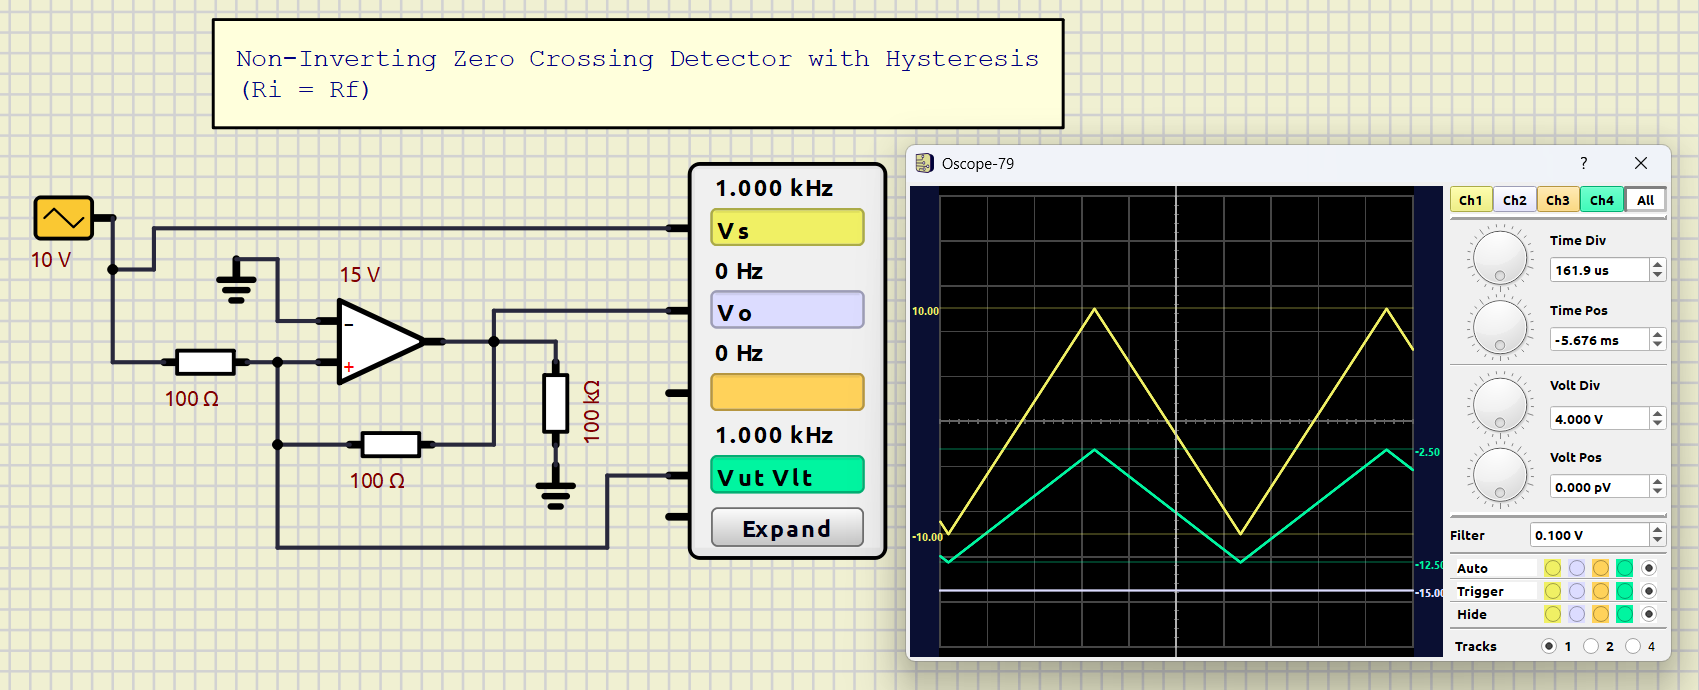
\includegraphics[width=0.5\linewidth]{images/NIZCD1.png}
        \caption{NIZCD with Hysteresis $R_1 = R_2$}
        \label{fig:enter-label}
        \end{figure}
    
    \item [b. ]$R_i < R_f$
        \begin{figure}[H]
        \centering
        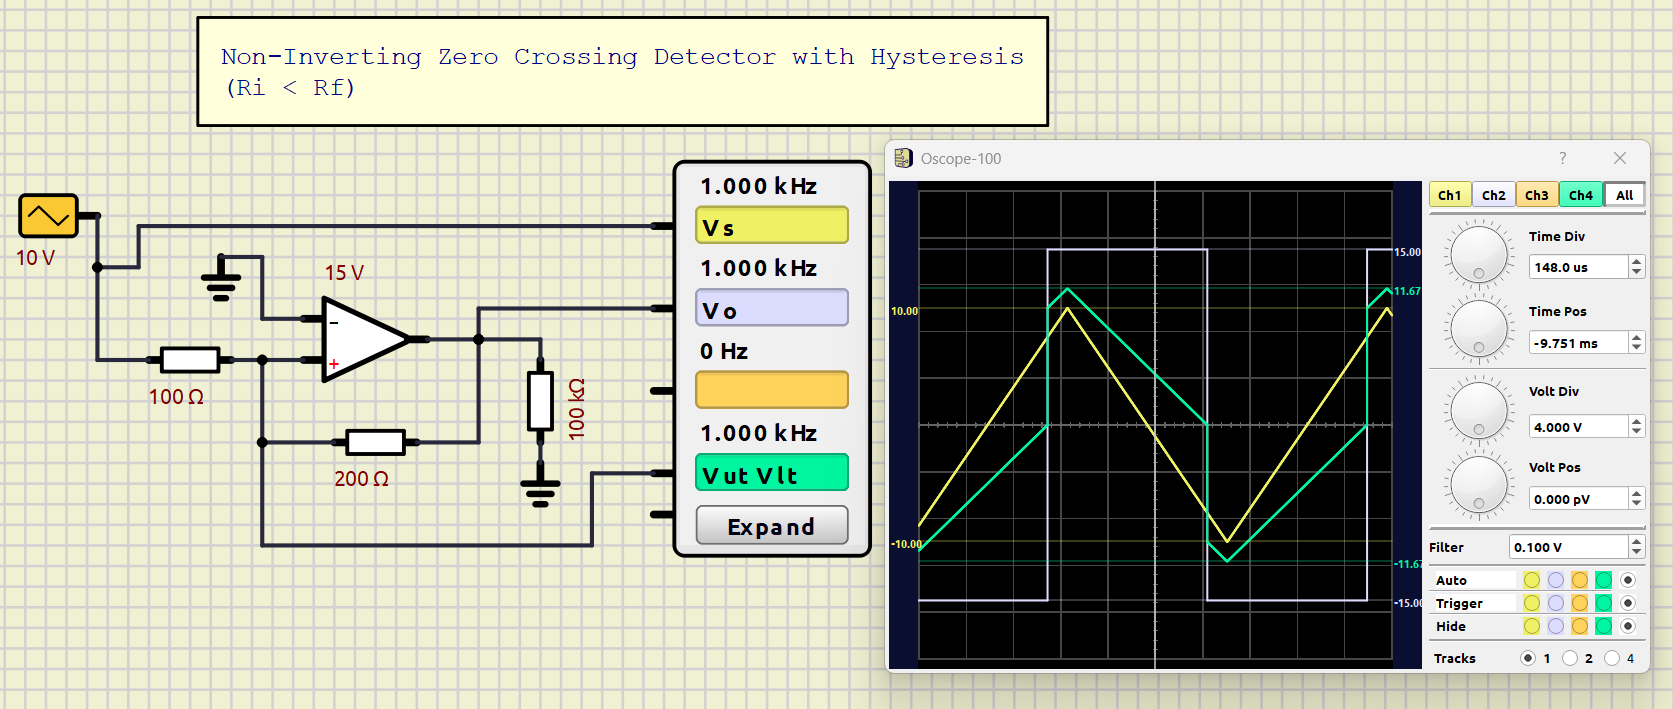
\includegraphics[width=0.5\linewidth]{images/NIZCD2.png}
        \caption{NIZCD with Hysteresis $R_1 < R_2$}
        \label{fig:enter-label}
        \end{figure}
    
    \item [c. ]$R_i > R_f$
        \begin{figure}[H]
        \centering
        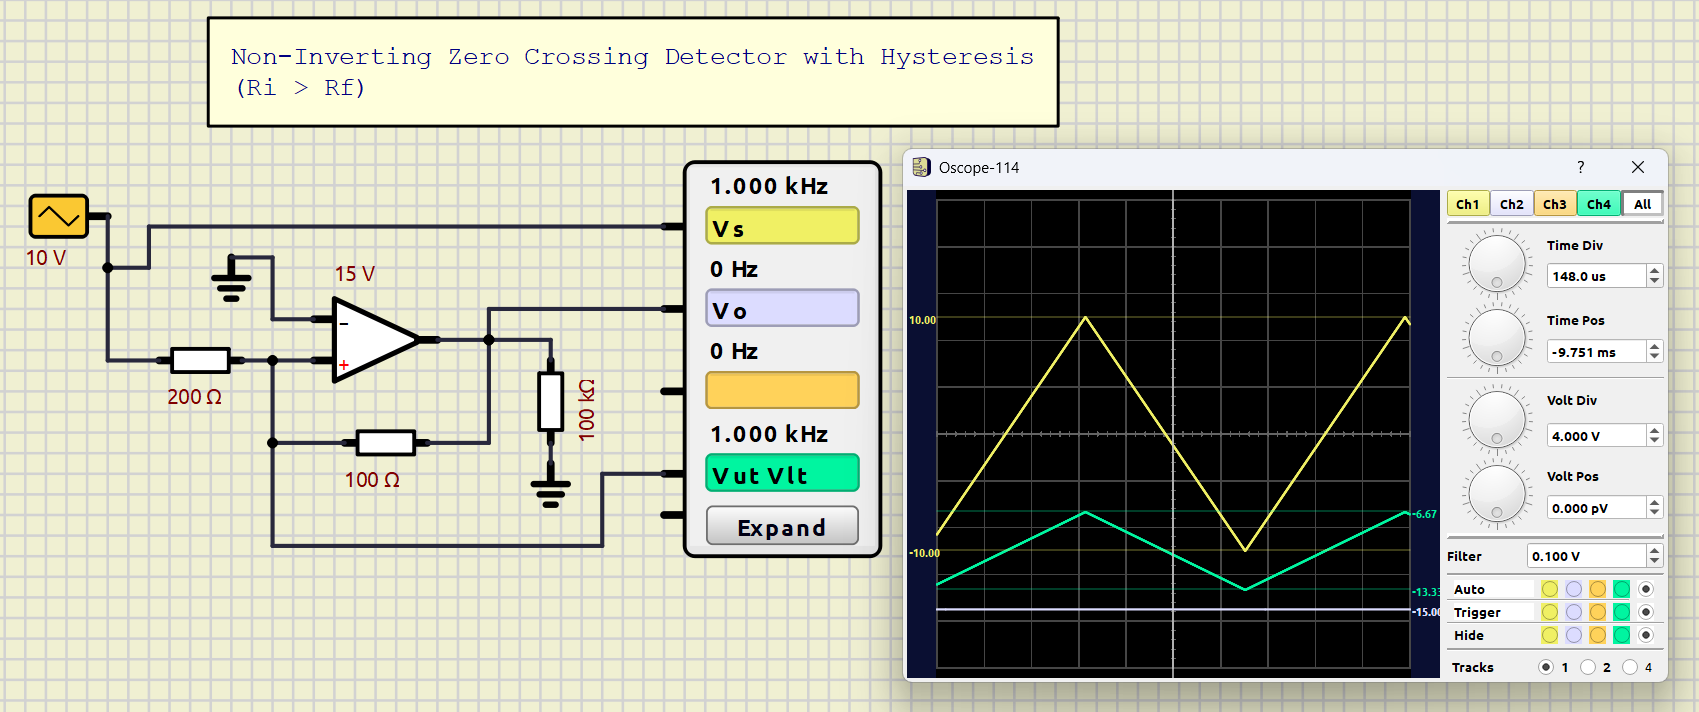
\includegraphics[width=0.5\linewidth]{images/NIZCD3.png}
        \caption{NIZCD with Hysteresis $R_1 > R_2$}
        \label{fig:enter-label}
        \end{figure}
    
\end{enumerate}

Pada simulasi rangkaian NIZCD ini, hasil pengujian menunjukkan karakteristik switching yang sangat bergantung pada perbandingan resistor input ($R_i$) dan feedback ($R_f$). Ketika nilai resistansi seimbang pada $R_i = R_f$, rangkaian tidak mengalami switching dan tegangan output ($V_o$) tertahan pada saturasi negatif ($-V_{sat}$) karena rentang ambang batasnya bergeser jauh ke area negatif ($-2.5V$ hingga $-12.5V$). Kondisi kegagalan serupa terjadi saat $R_i > R_f$, di mana output juga tetap mandek pada $-V_{sat}$ akibat threshold yang berada di level $-6.67V$ hingga $-13.33V$, sehingga amplitudo sinyal tidak mampu memicu transisi. Sebaliknya, proses transisi output dari $-V_{sat}$ ke $+V_{sat}$ hanya berhasil terjadi pada kondisi $R_i < R_f$, yang menghasilkan ambang batas sebesar $\pm 10V$. Namun pada skenario ini, bentuk gelombang output yang dihasilkan tidak berupa kotak sempurna, melainkan menunjukkan sedikit distorsi berupa kemiringan (ramp) tepat setelah melewati titik ambang. Kesimpulannya, pada konfigurasi NIZCD yang disimulasikan ini, operasi deteksi zero-crossing hanya dapat berjalan jika nilai resistor feedback dirancang lebih besar dari resistor input.

\begin{table}[H]
\centering
\caption{Perbandingan Karakteristik Rangkaian NIZCD dengan Variasi Resistor}
\label{tab:perbandingan_nizcd}
% \textwidth memaksa tabel lebarnya pas 100% dengan margin teks
% Kolom 'X' akan otomatis menghitung sisa ruang dan melakukan word-wrap
\begin{tabularx}{\textwidth}{|l|c|c|X|X|}
\hline
\textbf{Kondisi Resistansi} & \textbf{Threshold} & \textbf{Lebar} $V_H$ & \textbf{Respon Switching} & \textbf{Keterangan} \\ \hline
$R_i = R_f$ & $-2.5$V s.d. $-12.5$V & 10V & Tidak ada ($V_o = -V_{sat}$) & Gagal \textit{switching} \\ \hline
$R_i < R_f$ & $\pm 10$V & 20V & Berpindah ($-V_{sat}$ ke $+V_{sat}$) & Gelombang \textit{output} memiliki efek \textit{ramp} \\ \hline
$R_i > R_f$ & $-6.67$V s.d. $-13.33$V & 6.66V & Tidak ada ($V_o = -V_{sat}$) & Gagal \textit{switching} \\ \hline
\end{tabularx}
\end{table}

\section*{Kesimpulan}

Simulasi rangkaian Inverting (IZCD) dan Non-Inverting Zero Crossing Detector (NIZCD) membuktikan bahwa penambahan umpan balik positif (histerisis) sangat krusial untuk mencegah gangguan noise pada sinyal dengan cara menciptakan dua ambang batas tegangan ($V_{UT}$ dan $V_{LT}$). Pada IZCD, variasi rasio resistor hubungan yang jelas, di mana semakin dominan resistor feedback dibandingkan resistor ground, semakin lebar jendela histerisis yang dihasilkan, sehingga rangkaian makin kebal terhadap noise namun merespon lebih lambat. Sementara itu, simulasi NIZCD menunjukkan sifat operasional yang lebih kompleks, di mana rangkaian hanya mampu melakukan switching dengan baik jika resistor feedback dirancang lebih besar dari resistor input ($R_i < R_f$). Kegagalan memenuhi rasio ini menyebabkan ambang batas bergeser terlalu jauh sehingga output tertahan pada kondisi saturasi. Dengan demikian, penggunaan zero crossing detector dengan histerisis sangat bermanfaat namun perlu diperhatikan dalam merancangnya agar dapat beroperasi sesuai harapan.

\bibliographystyle{IEEEtran}
\bibliography{references}



\end{document}
